\documentclass[11pt]{article}
\usepackage{hyperref}
\usepackage{amsthm}
\usepackage{amsmath}
\usepackage{amsfonts}
\usepackage{tikz}
\usepackage{ wasysym }
\usepackage{fancyvrb}

\newtheorem{example}{Example}


\author{Group 3:  Hannah Jensen, Nicholas Jacob}
\title{Homework 1 Advanced Analytics and Metaheuristics}

\begin{document}
\maketitle
%{\Large
%%Change Document name to: Graded Homework 1\_Jacob\_Nicholas
%\noindent NAME:  Nicholas Jacob\\ 
%STUDENT ID: \# 113578513\\
%HOMEWORK NUMBER: 1\\
%COURSE: DSA 5113 Advanced Analytics and Metaheuristics\\ 
%SECTION: ONLINE\\SEMESTER: Spring 2024\\
%INSTRUCTOR:  DR. Charles Nicholson\\
% SCORE:}
%
%\newpage
\begin{enumerate}
\item To examine this story, I will create a table.  I will assume that a sinister lying creature always lies (even though we know this too not be true eg. politicians).  So really this lays out two circumstances with two options in each.  

\begin{tabular}{l|l|l}
&gurump&pvlork\\ \hline
Jedi&No& Yes\\
Jedi& Yes&No\\
Sith &No & Yes\\
Sith & Yes &No

\end{tabular}

Let's examine each with our information.  For the first we see that since Jedi would tell the truth, it cannot be.  You would not answer yes to a wrong question.  Similarly you cannot have the second either as you will tell the truth.  We move on to sith liars.  If gurump means No and asked if it means yes, a liar would reply in the affirmative.  This means the logic on the third one is correct.  We see the fourth is also possible.  Since gurump is yes and the creature lies, we would answer no or pvlork.  Thus we see that Baby Yoda is a liar.  We cannot however determine the meaning of gurump and pvlork.

\begin{tabular}{l|l|l|l}
&gurump&pvlork&Possible\\ \hline
Jedi&No& Yes& No\\
Jedi& Yes&No& No\\
Sith &No & Yes& Yes\\
Sith & Yes &No&Yes

\end{tabular}

\item I am going to state the problem here
\begin{quote}
A portfolio manager in charge of a bank portfolio has \$10 million to invest. The
securities available for purchase, as well as their respective quality ratings, maturities, and yields, are shown
in Table

\begin{tabular}{c|c|c|c|c|c|c}
Name & Type & QS Moody's & QS Banks& Years to M & Yield to m& After-tax yield\\\hline
A& Municipal& Aa &2& 9& 4.3\% &4.3\%\\
B& Agency& Aa& 2& 15& 5.4& 2.7\\
C& Government& Aaa &1 &4 &5.0 &2.5\\
D &Government &Aaa& 1& 3& 4.4& 2.2\\
E& Municipal &Ba &5 &2 &4.5 &4.5
\end{tabular}

The bank places the following policy limitations on the portfolio manager’s actions:
\begin{enumerate}
\item Government and agency bonds must total at least \$4 million.
\item  The average quality of the portfolio cannot exceed 1.4 on the bank’s quality scale. (Note that a low
number on this scale means a high-quality bond.)
\item  The average years to maturity of the portfolio must not exceed 5 years.
\end{enumerate}

\begin{enumerate}
\item Assuming that the objective of the portfolio manager is to maximize after-tax earnings and that the tax rate is 50 percent, what bonds should he purchase? 
\item If it became possible to borrow up to \$1 million at 5.5 percent before taxes, how should his selection be changed?
\end{enumerate}
\end{quote}

We'll start by stating the objective function, the return on investment after taxes:
\[
P(\vec x) = 0.043x_A + 0.027 x_B + 0.025 x_C + 0.022 x_D + 0.045 x_E
\]
This is the function that we wish to maximize.

Next we examine each of the constraints.
There is a total of 10 million to invest
\[
\sum x_i \leq 10 000 000
\]

  We need a total of at least 4 million in government and agency bonds so
\[
x_B + x_C+x_D \geq 4 000 000
\]
Then we want the average on the banks quality scale to not exceed 1.4 so
\[
\frac{2x_A +2x_B +x_C + x_D +5x_E}{\sum x_i} \leq 1.4
\]
We need to make this linear for AMPL (I learned after only a few minutes of face to keyboard)
\[
2x_A +2x_B +x_C + x_D +5x_E -1.4\sum x_i \leq 0
\]
Which simplifies to 
\[
0.6 x_A + 0.6 x_B -0.4 x_C -0.4 x_D +3.6 x_E \leq 0
\]
Lastly we wanted the average years to maturity to be less than 5 so 
\[
\frac{9x_A +15x_B +4x_C + 3x_D +2x_E}{\sum x_i} \leq 5
\]
This simplifies to 
\[
4x_A +10x_B -x_C -2 x_D -3x_E\leq 0
\]
With all of this we code it into AMPL and arrive at the output 

CPLEX 20.1.0.0: optimal solution; objective 298363.6364

3 dual simplex iterations (1 in phase I)

invest [*] :=

A  2181820

B        0

C  7363640

D        0

E   454545;

For the second part of the problem, we add the additional condition that we can take out a loan of up to 1 million at 5.5\%.  This will change our objective function
\[
P(\vec x) = 0.043x_A + 0.027 x_B + 0.025 x_C + 0.022 x_D + 0.045 x_E -0.055 x_{loan}
\]
The total amount invested must also change
\[
\sum x_i \leq 10 000 000 + x_{loan}
\]
Of course there are the restrictions on the loan too
\[
0\leq x_{loan}\leq 1 000 000
\]
The rest of the constraints remain unchanged.  Running it through AMPL arrives at the solution

CPLEX 20.1.0.0: optimal solution; objective 300700

5 dual simplex iterations (3 in phase I)

invest [*] :=

A  2400000

B        0

C  8100000

D        0

E    5e+05

borrowedFunds = 1e+06



\item I am going to state the problem here:

\begin{quote}
This exercise starts with a two-variable linear program similar in structure to the one of Sec-
tions 1.1 and 1.2, but with a quite different story behind it.
\begin{enumerate}
\item You are in charge of an advertising campaign for a new product, with a budget of \$1 million.
You can advertise on TV or in magazines. One minute of TV time costs \$20,000 and reaches 1.8
million potential customers; a magazine page costs \$10,000 and reaches 1 million. You must sign
up for at least 10 minutes of TV time. How should you spend your budget to maximize your audience? Formulate the problem in AMPL and solve it. Check the solution by hand using at least one of the approaches described in Section 1.1.

\item It takes creative talent to create effective advertising; in your organization, it takes three
person-weeks to create a magazine page, and one person-week to create a TV minute. You have
only 100 person-weeks available. Add this constraint to the model and determine how you should
now spend your budget.
\item Radio advertising reaches a quarter million people per minute, costs \$2,000 per minute, and
requires only 1 person-day of time. How does this medium affect your solutions?
\item How does the solution change if you have to sign up for at least two magazine pages? A maximum of 120 minutes of radio?
\end{enumerate}
\end{quote}

\begin{enumerate}
\item We begin by stating the objective function to maximize, eyeballs:
\[
z = 1.8 x + 1y
\]
Where $x$ is minutes of TV time, $y$ is pages in a magazine and $z$ is million viewers.  Next we set the two constraints, at least 10 minutes of TV and no more than \$1 million spent.
\[
\begin{array}{l}
x\geq 10\\
20 000 x + 10 000 y \leq 1 000 000
\end{array}
\]

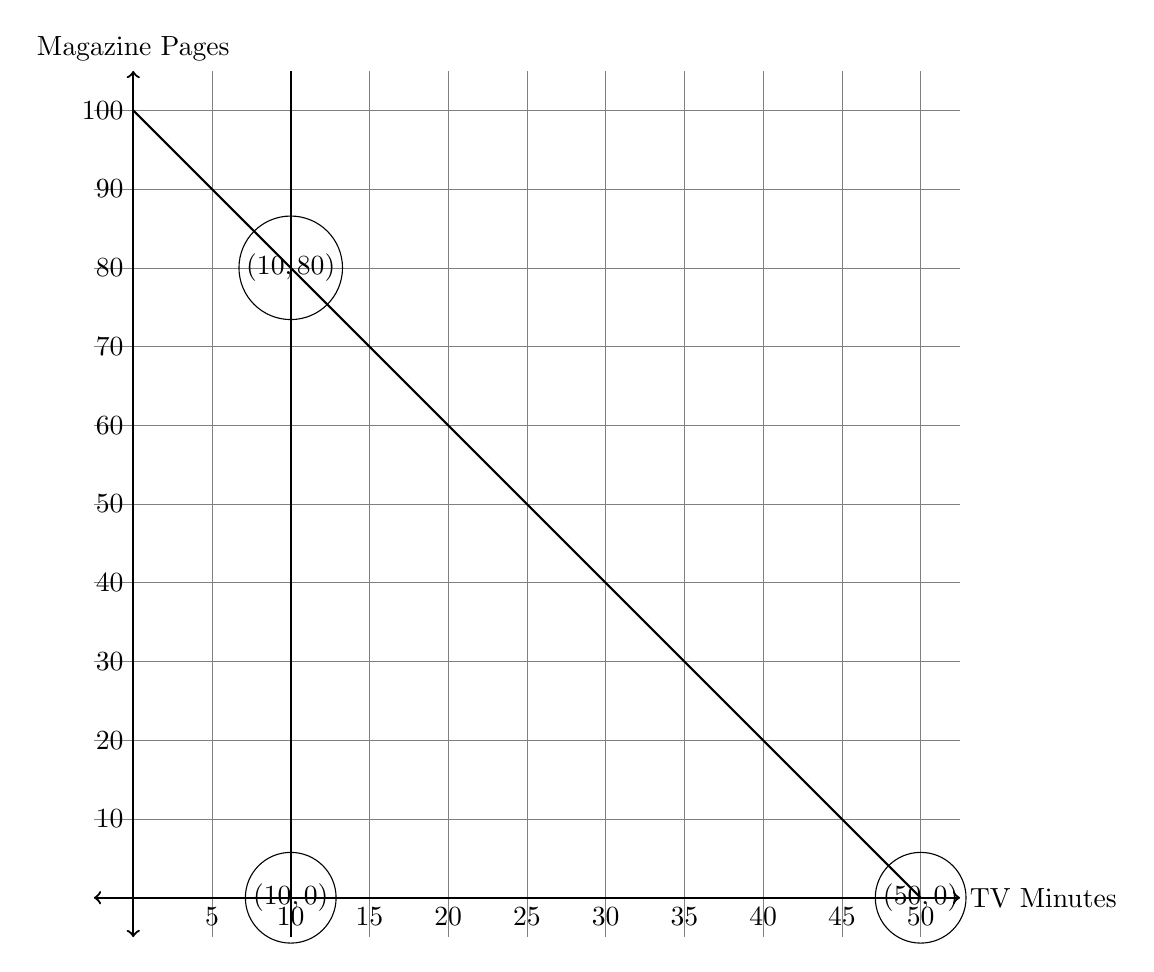
\begin{tikzpicture}
\draw[help lines] (-0.5,-0.5) grid (10.5,10.5);
\draw[thick][<->](0,10.5)--(0,-0.5);
\draw (0,10.5) node[above]{Magazine Pages};
\draw[thick][<->](10.5,0)--(-.5,0);
\draw (10.5,0) node[right]{TV Minutes};
\draw (0,1) node[left]{10};
\draw (0,2) node[left]{20};
\draw (0,3) node[left]{30};
\draw (0,4) node[left]{40};
\draw (0,5) node[left]{50};
\draw (0,6) node[left]{60};
\draw (0,7) node[left]{70};
\draw (0,8) node[left]{80};
\draw (0,9) node[left]{90};
\draw (0,10) node[left]{100};
\draw (1,0) node[below]{5};
\draw (2,0) node[below]{10};
\draw (3,0) node[below]{15};
\draw (4,0) node[below]{20};
\draw (5,0) node[below]{25};
\draw (6,0) node[below]{30};
\draw (7,0) node[below]{35};
\draw (8,0) node[below]{40};
\draw (9,0) node[below]{45};
\draw (10,0) node[below]{50};
\draw[thick] (2,10.5)--(2,-.50);
\draw[thick] (0,10)--(10,0);
\draw [nodes=draw, circle, inner sep=1.5pt]
    (2,8) node [] {$(10,80)$}
	(2,0) node []{$(10,0)$}
	(10,0) node [] {$(50,0)$};
\end{tikzpicture}

We see the corner points of the feasible set as possible solutions.  We are left to find the maximum:

\begin{tabular}{c|c|c}
Point& z & Optimizer\\\hline
$(10,80)$& 18+80 = 98&Max\\
$(10,0)$& 18+0 = 18&Min\\
$(50,0)$& 90+0 = 90&
\end{tabular}
\end{enumerate}

\end{enumerate}



\end{document}